\section{Introdução}

A modução é um tecnica que permite a transmissão de sinais analógicos ou digitais através de um meio físico, como o ar ou cabos.
Segundo \cite{b12}, a modulação AM é um processo que envolve a variação da amplitude de uma portadora de alta frequência em função de um sinal modulante, que contém a informação a ser transmitida. Essa técnica é amplamente utilizada em sistemas de comunicação, como rádio e televisão, devido à sua simplicidade e eficácia na transmissão de sinais analógicos.


\subsection{Modulação AM-DSB-SC (Double Sideband Suppressed Carrier)}
A modulação AM-DSB (Double Sideband) é uma forma de modulação em que a portadora e as duas laterais (superior e inferior) são transmitidas. Esse tipo de modulação consiste em multiplicar o sinal de informação por uma portadora, como o sinal mensagem é de banda limitada, isto é, se o sinal $m(t)$ admite transformada de fourier, então $M(f) = 0$ para $|f| > W$, onde $W$ é a largura de banda do sinal.
Como a mensagem tem sua representação espectral, é possivel deslocar a mensagem para uma nova frequência utilizando a propriedade de modulação da transformada de Fourier, que nos diz que a multiplicação no domínio do tempo por uma exponencial complexa resulta em um deslocamento espectral no domínio da frequência. Multplicando o sinal de informação $m(t)$ por uma portadora $c(t) = A_{c} \cos(2 \pi f_{c} t)$, temos:
\begin{equation}
    s(t) = m(t) c(t) = A_{c} m(t) \cos(2 \pi f_{c} t)
\end{equation}

onde $A_{c}$ é a amplitude da portadora e $f_{c}$ é a frequência da portadora. Podemos expandir a expressão acima utilizando a identidade trigonométrica $\cos(x) = \frac{e^{jx} + e^{-jx}}{2}$, resultando em:

\begin{equation}
    s(t) = \frac{A_{c}}{2} m(t) e^{j 2 \pi f_{c} t} + \frac{A_{c}}{2} m(t) e^{-j 2 \pi f_{c} t}
\end{equation}

pode-se aplicar a transformada de Fourier em ambos os lados da equação, resultando em:

\begin{equation}
    S(f) = \frac{A_{c}}{2} (M(f - f_{c}) + M(f + f_{c}))
\end{equation}
Por exemplo, para uma mensagem $\cos(2\pi f_{m} t)$ com frequência $f_{m} = 100\,\text{Hz}$, uma portadora $\cos(2\pi f_{c} t)$ de $f_{c} = 1\,\text{kHz}$ com amplitude $A_{c} = 1$, realizando a modulação AM-DSB, os espectros para a mensagem, portadora e sinal modulado são mostrados nas Figuras~\ref{fig:espectro_mensagem}, \ref{fig:espectro_portadora} e \ref{fig:espectro_modulado}, respectivamente. O espectro do sinal modulado AM-DSB apresenta duas bandas laterais, uma superior e outra inferior, que contêm a mesma informação, além da portadora.

\begin{figure}[h]
    \centering
    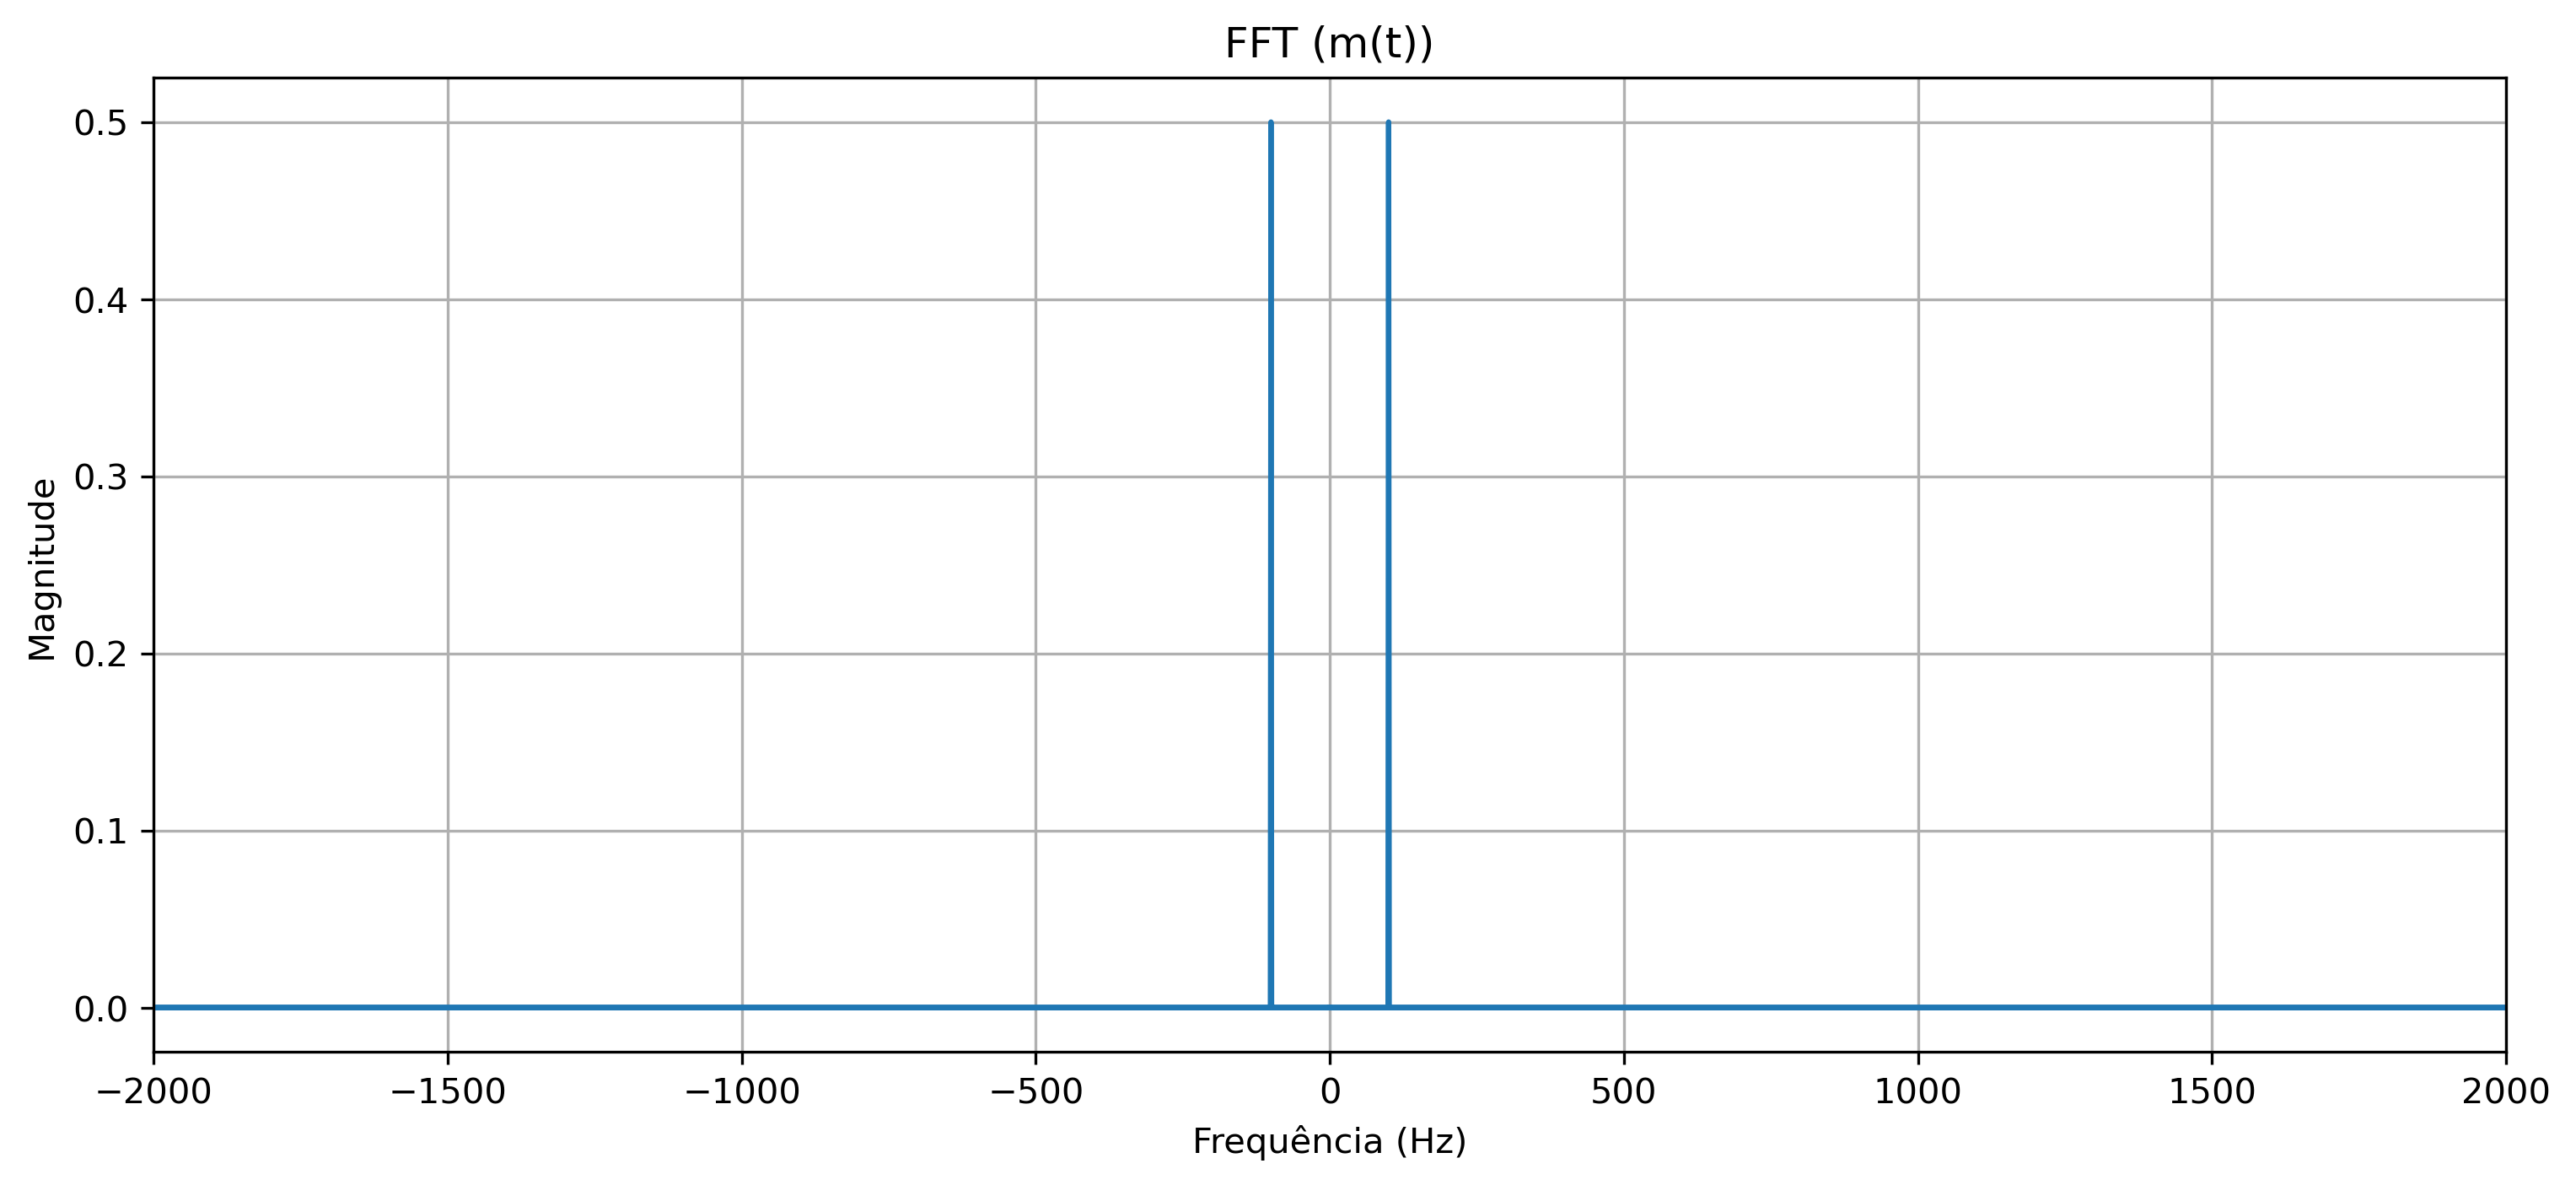
\includegraphics[width=0.5\textwidth]{images/FFT (m(t))_full.png}
    \caption{Espectro do sinal de mensagem. Fonte: Autor.}
    \label{fig:espectro_mensagem}
    \centering
\end{figure}

\begin{figure}[h]
    \centering
    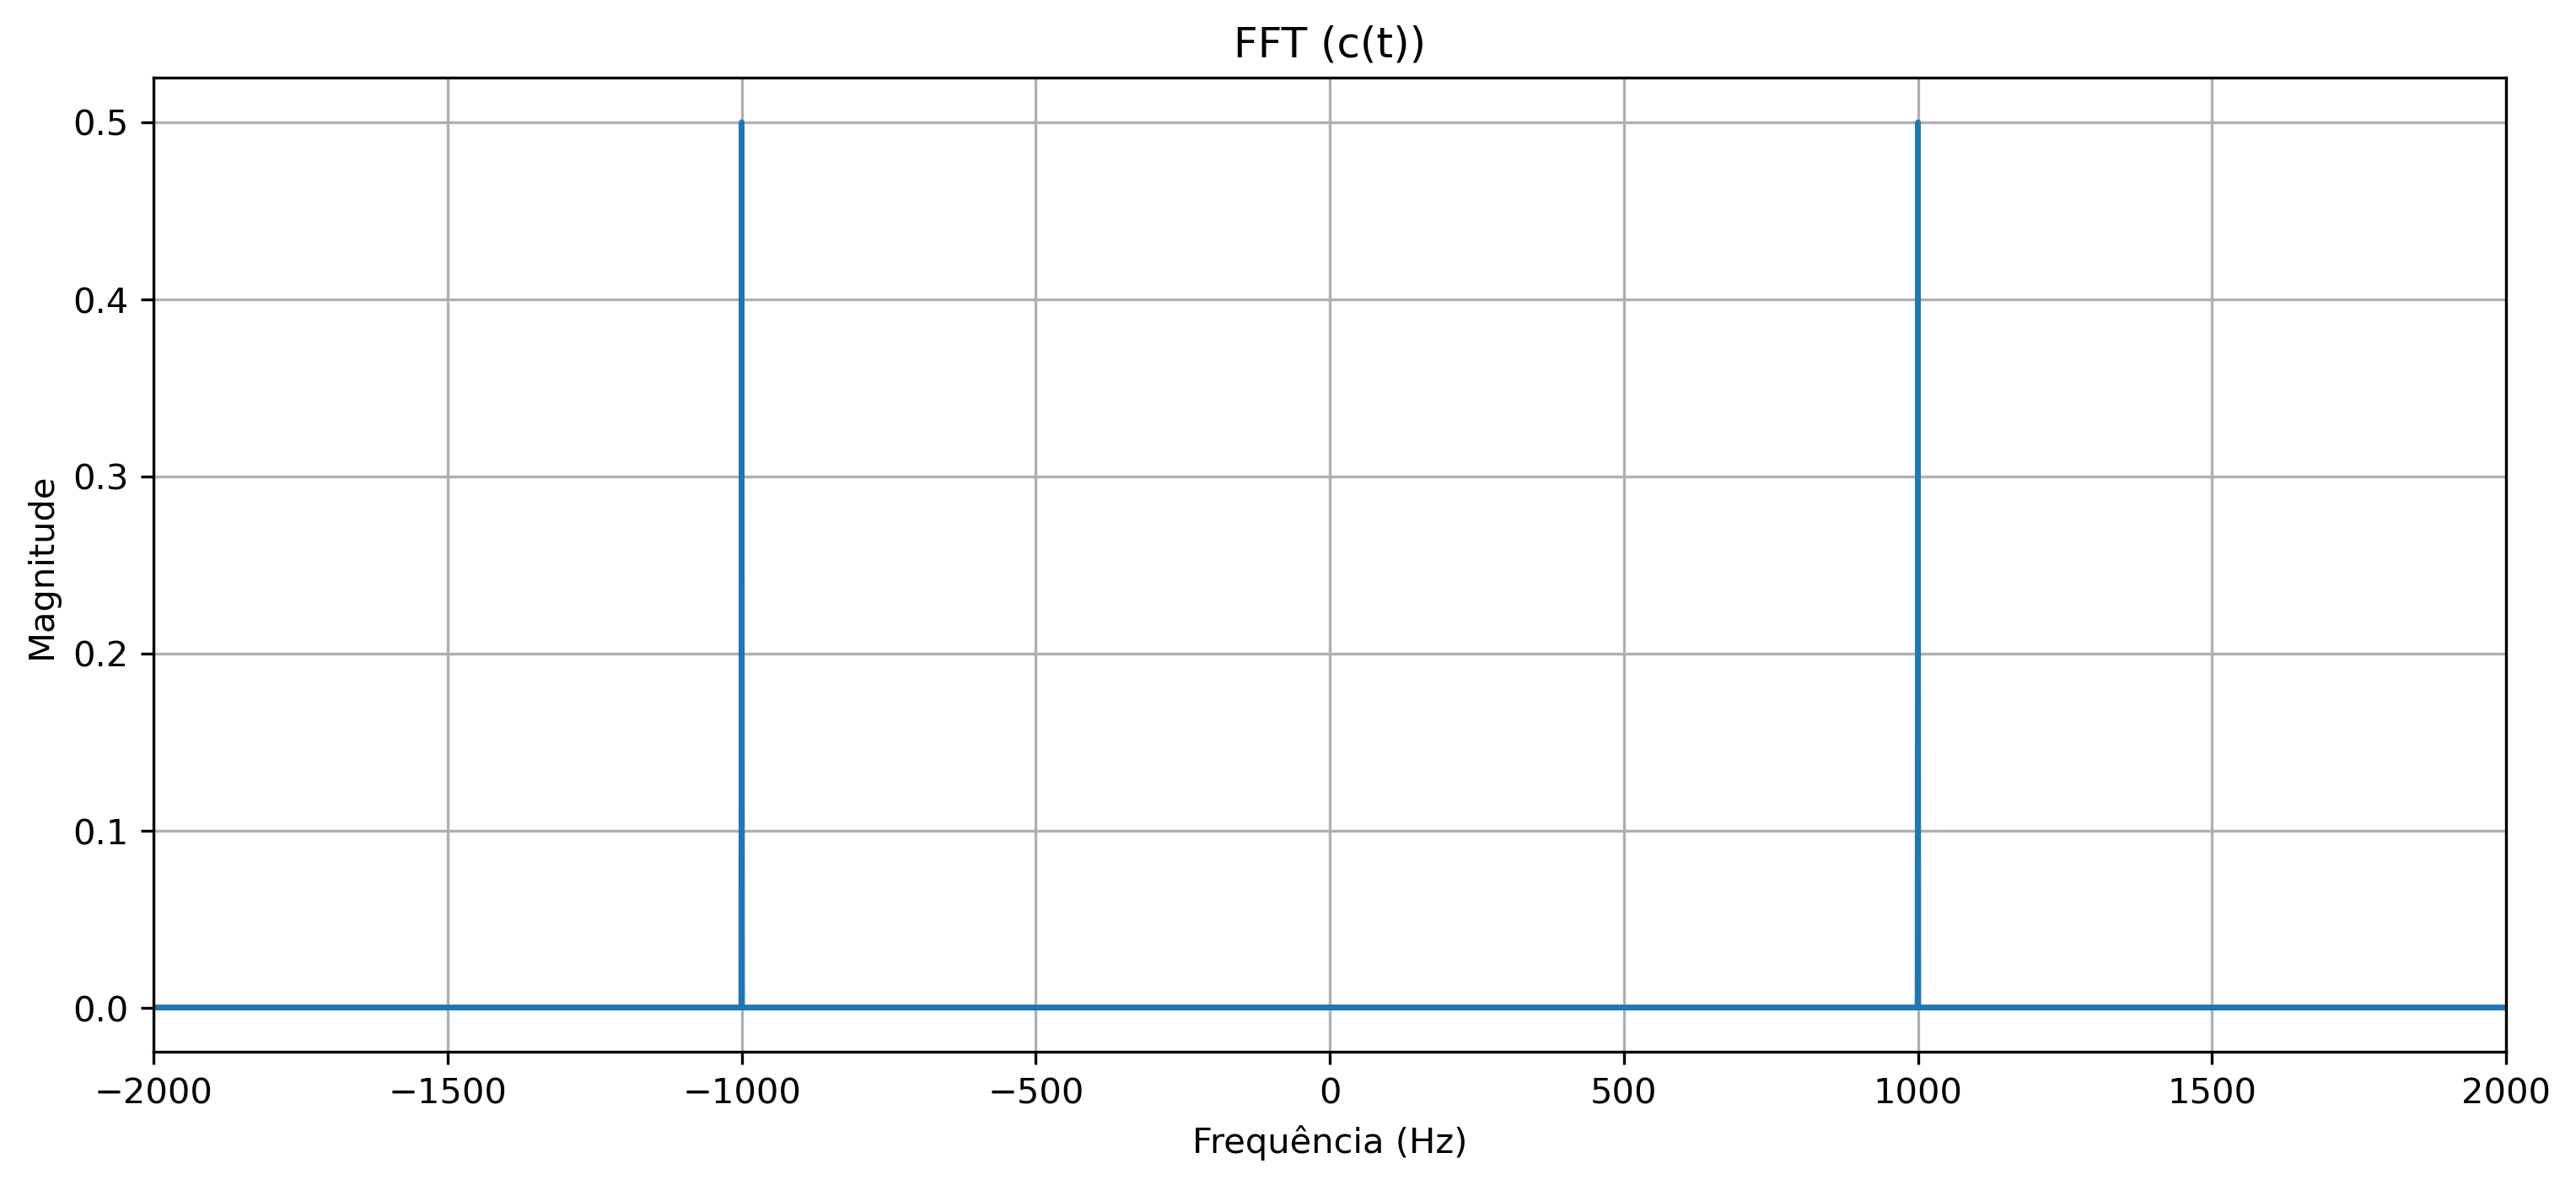
\includegraphics[width=0.5\textwidth]{images/FFT (c(t))_full.png}
    \caption{Espectro da portadora. Fonte: Autor.}
    \label{fig:espectro_portadora}
    \centering
\end{figure}

\begin{figure}[h]
    \centering
    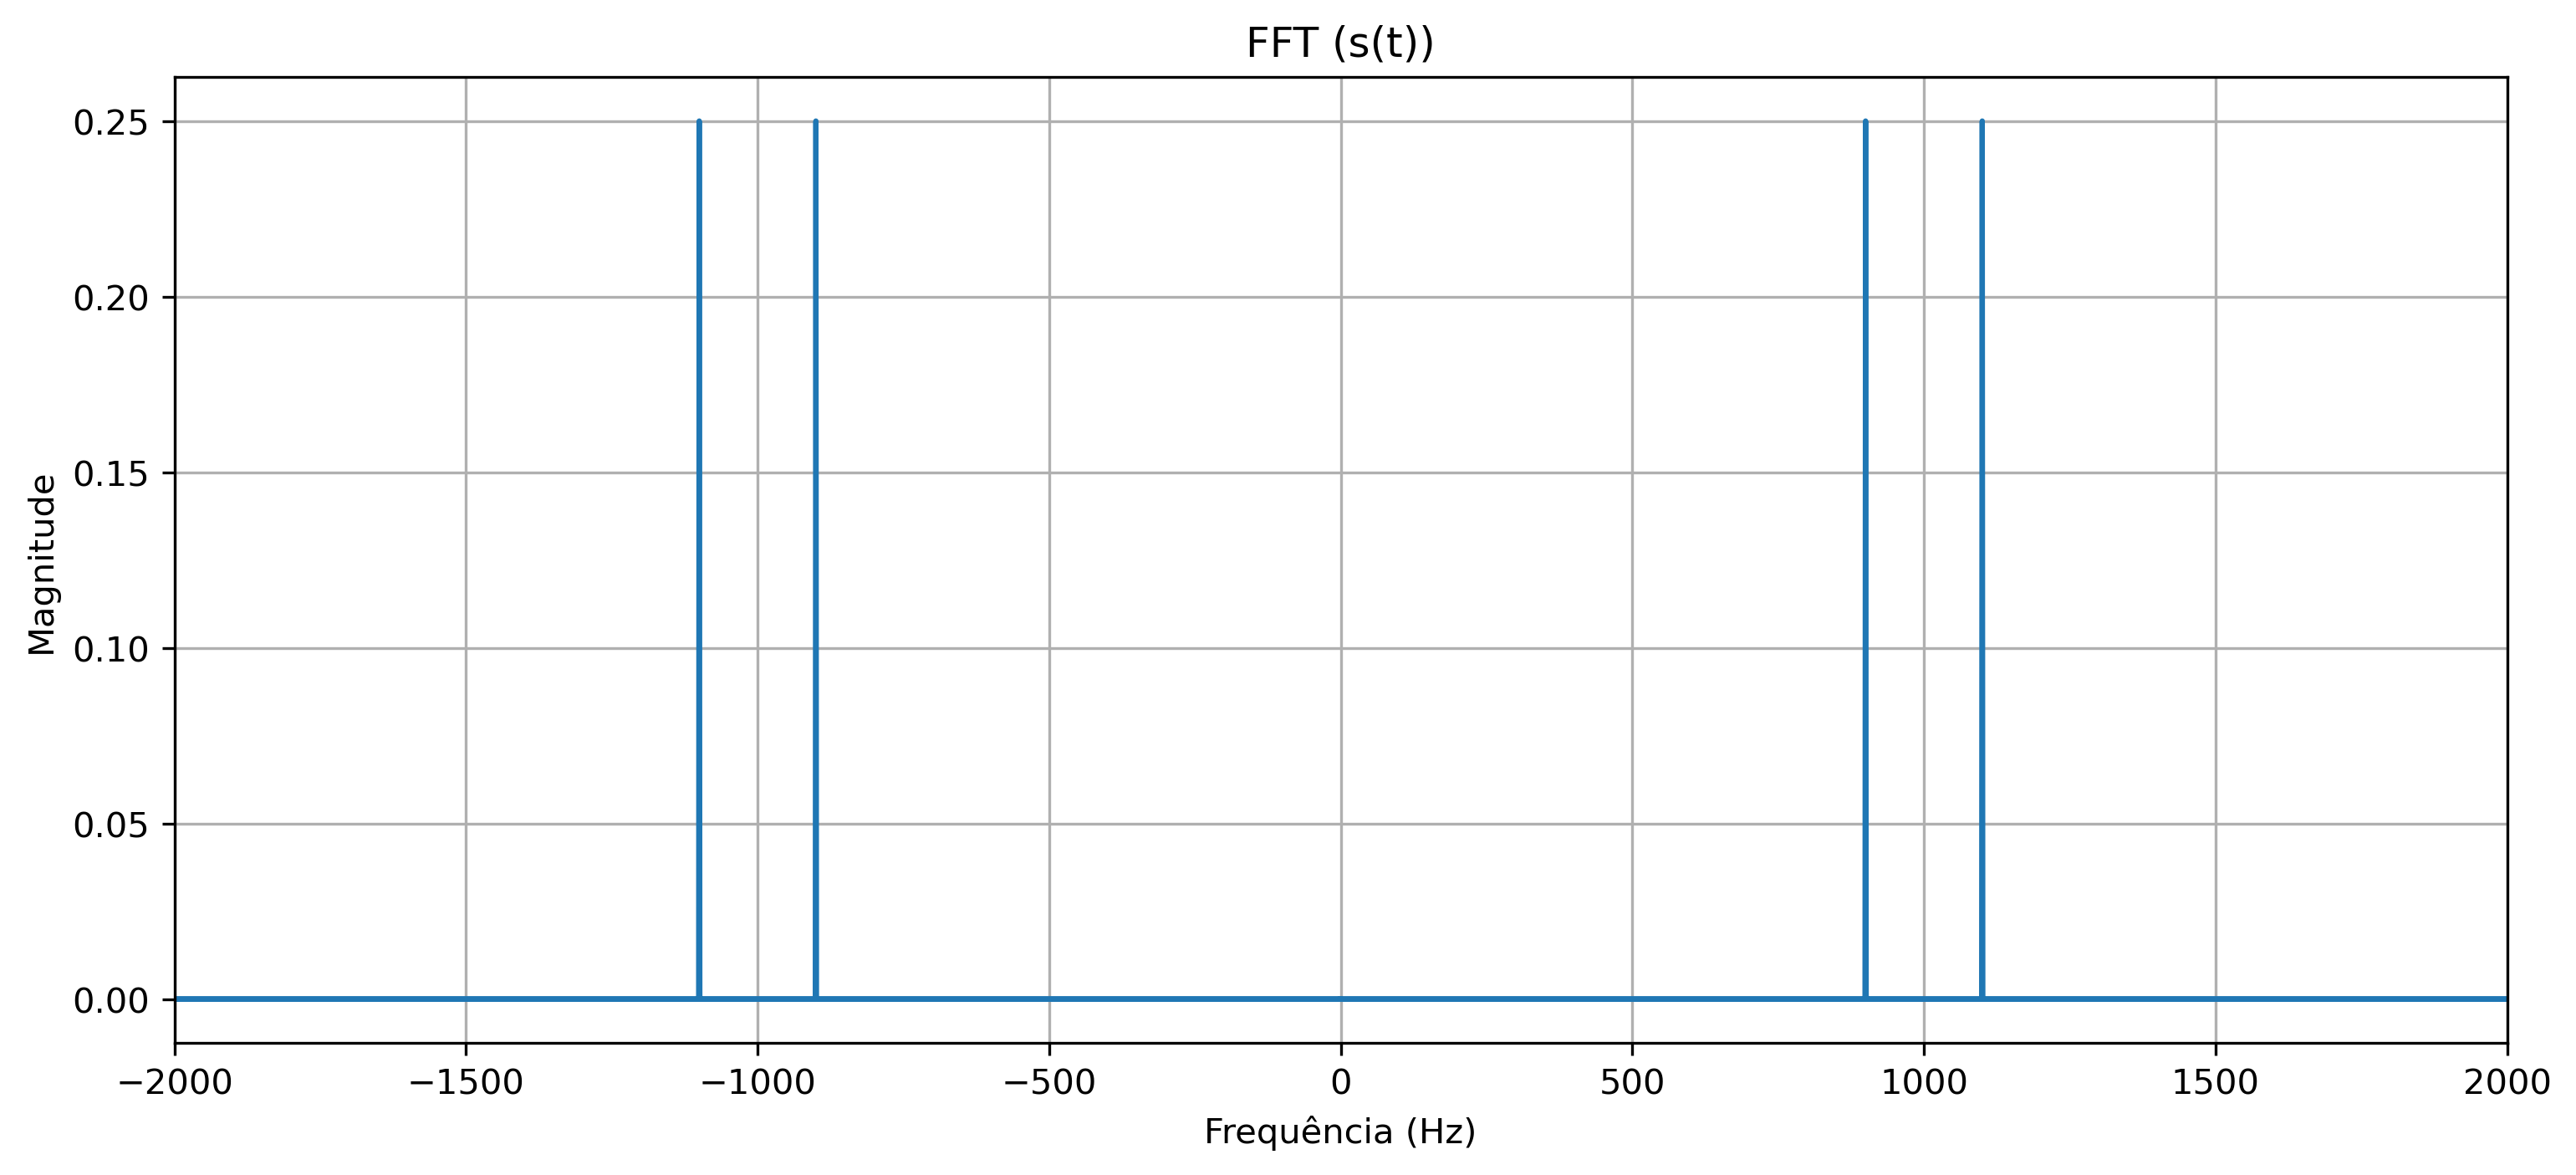
\includegraphics[width=0.5\textwidth]{images/FFT (s(t))_full.png}
    \caption{Espectro do sinal modulado AM-DSB. Fonte: Autor.}
    \label{fig:espectro_modulado}
    \centering
\end{figure}


O diagrama de blocos da modulação AM-DSB é apresentado na Figura \ref{fig:modulacao_am}, onde o sinal de informação $m(t)$ é multiplicado pela portadora $c(t)$, resultando no sinal modulado $s(t)$. A demodulação do sinal AM-DSB pode ser realizada utilizando um detector de envoltória, que recupera o sinal de informação original a partir do sinal modulado.

\begin{figure}[h]
    \centering
    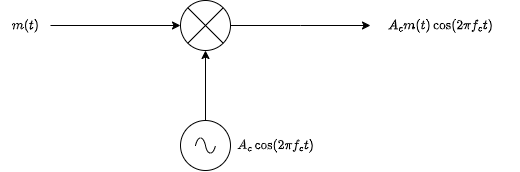
\includegraphics[width=0.5\textwidth]{images/modulacao_am.png}
    \caption{Diagrama de blocos da modulação AM-DSB. Fonte: Autor.}
    \label{fig:modulacao_am}
\end{figure}


Podemos demostrar os resultados a partir da transformada de Fourier, onde a transformada de Fourier do sinal modulado $m(t)$ é dada por:

\begin{equation}
    M(f) = \frac{1}{2} \left( \delta (f - 100) + \delta (f + 100) \right)
\end{equation}

substituindo na equação (3), temos:

\begin{align}
    S(f) = \frac{1}{4} \big(
        &\ \delta (f - 100 - 1000) + \delta (f + 100 - 1000) \notag \\
        &+ \delta (f - 100 + 1000) + \delta (f + 100 + 1000)
    \big)
\end{align}

Conforme mostrado no espectro \ref{fig:espectro_modulado}, a portadora é suprimida.


\subsection{demodulação AM-DSB-SC (Double Sideband Suppressed Carrier)}

A demodulação AM-DSB-SC é um processo que visa recuperar o sinal de informação original a partir do sinal modulado. O método mais comum para realizar essa demodulação é o uso de um multiplicador, que multiplica o sinal modulado por uma cópia da portadora. Esse processo resulta em um sinal que contém a informação original, mas também inclui uma componente de alta frequência que deve ser filtrada.

\begin{equation}
    s(t) = m(t) c(t) = A_{c} m(t) \cos(2 \pi f_{c} t)
\end{equation}

\begin{equation}
    y(t) = s(t) c(t) \cos(2 \pi f_{c}t)= A_{c} m(t) \cos(2 \pi f_{c} t)^{2}
\end{equation}

Linarizando o coseno, tempos:

\begin{equation}
    r(t) = \frac{A_{c}}{2} m(t) + \frac{A_{c}}{2} m(t) \cos(4 \pi f_{c} t)
\end{equation}

A transformada de Fourier do sinal demodulado $r(t)$ é dada por:

\begin{equation}
    Y(f) = \frac{A_{c}}{2} M(f) + \frac{A_{c}}{2} M(f - 2 f_{c}) + \frac{A_{c}}{2} M(f + 2 f_{c})
\end{equation}

Aplicando um filtro passa-baixa com largura de banda $W$ para eliminar a componente de alta frequência, obtemos o sinal de informação original:

\begin{equation}
    Y_{LPF}(f) = \frac{A_{c}}{2} M(f)
\end{equation}

O sinal é recuperado com uma amplitude reduzida, o que pode ser compensado por um amplificador. O diagrama de blocos da demodulação AM-DSB-SC é apresentado na Figura \ref{fig:demodulacao_am}, onde o sinal modulado $s(t)$ é multiplicado pela portadora $c(t)$, resultando no sinal demodulado $r(t)$. Em seguida, um filtro passa-baixa é aplicado para recuperar o sinal de informação original.

\begin{figure}[h]
    \centering
    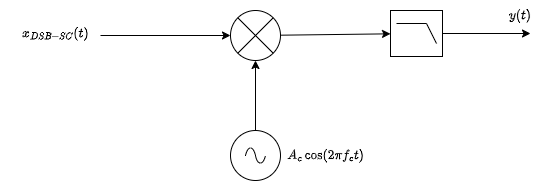
\includegraphics[width=0.5\textwidth]{images/demodulacao_am.png}
    \caption{Diagrama de blocos da demodulação AM-DSB-SC. Fonte: Autor.}
    \label{fig:demodulacao_am}
\end{figure}

Um dos principais desafios da modulação em amplitude com portadora suprimida (DSB-SC) é a necessidade de sincronização de fase entre o sinal modulado e a portadora na demodulação. Caso haja um desvio de fase entre a portadora original e a gerada no receptor, o sinal demodulado apresentará distorções significativas. Para mitigar esse problema, uma abordagem comum é transmitir um tom piloto juntamente com o sinal modulado. Esse tom é uma pequena fração da portadora original, inserida com baixa amplitude, e pode ser isolado no receptor por meio de um filtro de banda estreita. No entanto, a presença do tom piloto implica que a portadora não está totalmente suprimida, o que descaracteriza a modulação como DSB-SC pura.

Outra alternativa mais robusta é o uso de um PLL (Phase-Locked Loop), um circuito que sincroniza automaticamente a fase da portadora local com a fase do sinal modulado recebido. O PLL ajusta continuamente a frequência e a fase do oscilador local, permitindo uma demodulação mais precisa mesmo na presença de ruídos e desvios de fase. A Figura \ref{fig:demodulacao_am_pll} ilustra o esquema de demodulação utilizando PLL.

\begin{figure}[h]
    \centering
    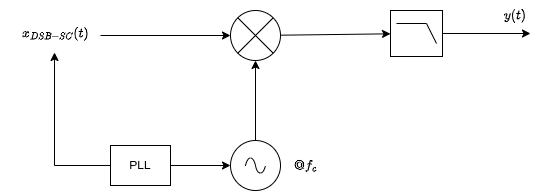
\includegraphics[width=0.5\textwidth]{images/demodulacao_am_pll.png}
    \caption{Diagrama de blocos da demodulação AM-DSB-SC com PLL. Fonte: Autor.}
    \label{fig:demodulacao_am_pll}
    \centering
\end{figure}

\subsection{Modulação AM Convencional}

Um sinal AM convencional consiste em uma componente portadora de grande amplitude, além do sinal modulado em DSB-AM. O sinal transmitido pode ser expresso matematicamente como:

\begin{equation}
u(t) = A_c[1 + m(t)] \cos(2\pi f_c t)
\end{equation}

onde $m(t)$ representa o sinal mensagem, o qual deve satisfazer a condição $|m(t)| \leq 1$ para garantir que a envoltória do sinal modulado permaneça sempre positiva. A componente $A_c m(t) \cos(2\pi f_c t)$ constitui o sinal DSB-AM, enquanto $A_c \cos(2\pi f_c t)$ representa a portadora.

A Figura~\ref{fig:am_envoltoria} ilustra a envoltória do sinal modulado:

\begin{figure}[h]
    \centering
    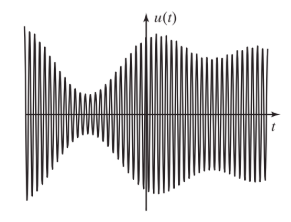
\includegraphics[width=0.3\textwidth]{images/envoltoria.png}
    \caption{Envoltoria do Sinal AM. Fonte: Proakis}
    \label{fig:am_envoltoria}
    \centering
\end{figure}

Na prática, o sinal $m(t)$ é escalado para garantir que sua magnitude esteja sempre dentro do intervalo desejado. Uma forma conveniente de fazer isso é expressar:

\begin{equation}
m(t) = a m_n(t)
\end{equation}

em que $m_n(t)$ é o sinal normalizado tal que seu valor mínimo é $-1$, definido por:

\begin{equation}
m_n(t) = \frac{m(t)}{\max |m(t)|}
\end{equation}

Nesse caso, o fator de escala $a$ é chamado de índice de modulação, sendo um valor constante geralmente menor que 1. Como $|m_n(t)| \leq 1$ e $0 < a < 1$, tem-se que $1 + a m_n(t) > 0$, evitando sobremodulação. Assim, o sinal modulado pode ser reescrito como:

\begin{equation}
u(t) = A_c[1 + a m_n(t)] \cos(2\pi f_c t)
\end{equation}

\subsubsection*{Espectro do Sinal AM Convencional}

Se $m(t)$ possui transformada de Fourier $M(f)$, o espectro do sinal modulado $u(t)$ será:

\begin{equation}
U(f) = \mathcal{F}\{A_c a m_n(t) \cos(2\pi f_c t)\} + \mathcal{F}\{A_c \cos(2\pi f_c t)\}
\end{equation}

\begin{equation}
U(f) = \frac{A_c a}{2}[M_n(f - f_c) + M_n(f + f_c)] + \frac{A_c}{2}[\delta(f - f_c) + \delta(f + f_c)]
\end{equation}

Portanto, o espectro de um sinal AM convencional ocupa uma largura de banda que é o dobro da largura de banda do sinal mensagem. A Figura \ref{fig:am_espectro}  apresenta o espectro $M(f)$.

\begin{figure}[h]
\centering
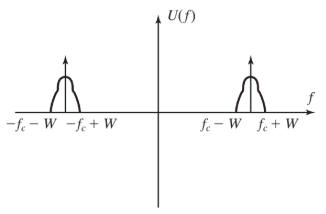
\includegraphics[width=0.3\textwidth]{images/espectro_am.png}
\caption{Sinal AM convencional no domínio do tempo e da frequência. Fonte: Proakis} 
\label{fig:am_espectro}
\end{figure}

A geração de um sinal AM pode ser feita utilziando um gerador de onda quadrada e um filtro passa banda

\begin{figure}[h]
\centering
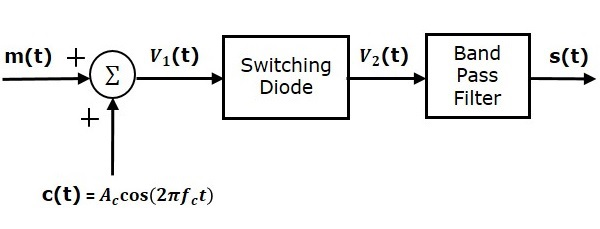
\includegraphics[width=0.3\textwidth]{images/blocos_amd_con.png}
\caption{Sinal no dominio da frequencia. Fonte: Tutorialspoint} 
\label{fig:diagrama_blocos_am_convencional}
\end{figure}

\subsection{Demodulação AM}

A demodulação de sinais AM convencionais pode ser realizada de forma simples utilizando um detector de envoltória, dispensando a necessidade de demodulação síncrona. O detector de envoltória é composto basicamente por um diodo e um circuito RC (filtro passa-baixa), como ilustrado na Figura~\ref{fig:circuito_demodulador_am}.

\begin{figure}[h]
\centering
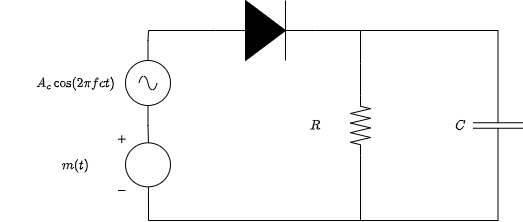
\includegraphics[width=0.3\textwidth]{images/demodulacao_am_circuito.png}
\caption{Circuito do detector de envoltória para demodulação AM. Fonte: Autor} 
\label{fig:circuito_demodulador_am}
\end{figure}

O funcionamento é simples: durante o semiciclo positivo do sinal de entrada, o diodo conduz e o capacitor carrega até o valor de pico do sinal. Quando o sinal cai abaixo da tensão do capacitor, o diodo se bloqueia e o capacitor descarrega lentamente pelo resistor, acompanhando a envoltória do sinal modulado. O filtro RC elimina as componentes de alta frequência, recuperando o sinal mensagem. Para remover a componente DC basta usar um transformador.

A escolha do valor da constante de tempo $RC$ é fundamental: se $RC$ for muito pequeno, o capacitor descarrega rapidamente e não acompanha a envoltória; se for muito grande, a descarga é lenta e o sinal fica distorcido. O valor ideal de $RC$ deve satisfazer:
\[
\frac{1}{f_c} \ll RC \ll \frac{1}{W}
\]
onde $f_c$ é a frequência da portadora e $W$ a largura de banda do sinal mensagem. A Figura~\ref{fig:envoltoria_rc_errado} mostra o efeito de um $RC$ inadequado, enquanto a Figura~\ref{fig:envoltoria_rc_correto} ilustra o funcionamento correto.

\begin{figure}[h]
\centering
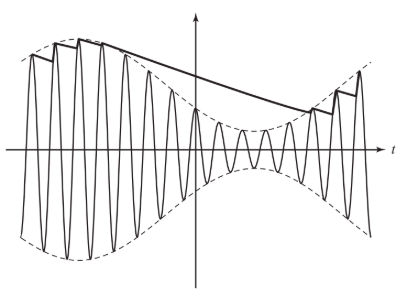
\includegraphics[width=0.3\textwidth]{images/envoltoria_rc_errado.png}
\caption{Envoltória para um RC fora do intervalo ideal. Fonte: \cite{b13}} 
\label{fig:envoltoria_rc_errado}
\end{figure}

\begin{figure}[h]
\centering
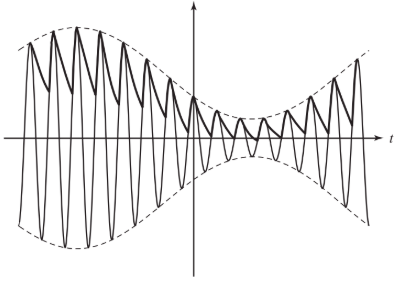
\includegraphics[width=0.3\textwidth]{images/envoltoria_rc_correto.png}
\caption{Envoltória para um RC dentro do intervalo ideal. Fonte: \cite{b13}} 
\label{fig:envoltoria_rc_correto}
\end{figure}



\section{Sincronismo de Fase em AM-DSB-SC}

A demodulação coerente do sinal AM-DSB-SC exige perfeito sincronismo entre a fase da portadora do transmissor ($\phi_c$) e do oscilador local no receptor ($\hat{\phi}_c$). O processo pode ser descrito por:

\subsection{Modulação}
O sinal modulado é gerado por:
\begin{equation}
    s(t) = m(t) \cdot A_c \cos(2\pi f_c t + \phi_c)
\end{equation}
onde:
\begin{itemize}
    \item $m(t)$: sinal da mensagem
    \item $A_c$: amplitude da portadora
    \item $f_c$: frequência da portadora
    \item $\phi_c$: fase da portadora no transmissor
\end{itemize}

\subsection{Demodulação}
O receptor multiplica pelo oscilador local:
\begin{equation}
    \hat{c}(t) = \cos(2\pi f_c t + \hat{\phi}_c)
\end{equation}

Resultando em:
\begin{equation}
    y(t) = s(t) \cdot \hat{c}(t) = \frac{A_c}{2} m(t) \left[ \cos(\phi_c - \hat{\phi}_c) + \cos(4\pi f_c t + \phi_c + \hat{\phi}_c) \right]
\end{equation}

Após filtragem passa-baixa:
\begin{equation}
    y_{\text{final}}(t) = \frac{A_c}{2} m(t) \cos(\Delta \phi)
\end{equation}
onde $\Delta \phi = \phi_c - \hat{\phi}_c$ é o erro de fase.

\subsection{Efeitos do Erro de Fase}
\begin{itemize}
    \item \textbf{Sincronismo perfeito} ($\Delta \phi = 0^\circ$):
    \begin{equation}
        y_{\text{final}}(t) = \frac{A_c}{2} m(t)
    \end{equation}
    
    \item \textbf{Erro de fase genérico}:
    \begin{equation}
        y_{\text{final}}(t) = \frac{A_c}{2} m(t) \cos(\Delta \phi)
    \end{equation}
    
    \item \textbf{Caso crítico} ($\Delta \phi = 90^\circ$):
    \begin{equation}
        y_{\text{final}}(t) = 0
    \end{equation}
\end{itemize}
